\documentclass[../statistics.tex]{subfiles}

\begin{document}
%%%%%%%%%%%%%%%%%%%%%%%%%%%%%%%%%%%%%%%%%%%%%%%%%%%%%%%%%%%%%%%%%%%% Likelihood
\chapter{Likelihood}%
\label{sec:likelihood}
[References:
\href{https://en.wikipedia.org/wiki/Likelihood_function}{Likelihood Function},
\href{https://en.wikipedia.org/wiki/Bayes'_theorem}{Bayes' Theorem}]

\noindent
The likelihood expresses how likely particular values of statistical model
parameters are for a given sample of data. It is \textbf{equal} to the joint
probability distribution of a random sample, but with the random variable fixed
at the given observations.

The likelihood describes a hypersurface whose peak, if it exists, represents
the combination of model parameter values that \textbf{maximize} the
probability of drawing the sample obtained.
%
\begin{align*}
  \text{Posterior Probability} = \frac{\text{Likelihood} \cdot \text{Prior Probability}}{\text{Evidence}}
\end{align*}


\section{Discrete Probability Distribution}%
\label{sec:discrete_probability_distribution}
Let $X$ be a discrete random variable with probability mass function $p$
depending on a parameter $\theta$, then the likelihood function is
%
\begin{align*}
  \mathcal{L}(\theta \vert x) = p_{\theta}(x) = P_{\theta}(X = x).
\end{align*}
%
\textbf{Example:} Consider a statistical model of a coin flip.
$p_H \in [0.0, 1.0]$ expresses the ``fairness'' of the coin, which is the
probability that a coin lands heads up (``H'') when tossed. For a perfectly
fair coin, $p_H = 0.5$. In a case that two heads observed in two tosses
(``HH'') and assuming each successive coin flip is i.i.d., then
%
\begin{align*}
  P(\text{HH} \vert p_H = 0.5) = 0.5^2 = 0.25.
\end{align*}
%
Hence, given this observed data HH, the likelihood that $p_H = 0.5$ is 0.25:
%
\begin{align*}
  \mathcal{L}(p_H = 0.5 \vert \text{HH}) = 0.25.
\end{align*}
%
This is \textbf{NOT} the same as saying that the probability that $p_H = 0.5$
is 0.25 given the observation HH\@.
%
\begin{figure}[htpb]
  \centering
  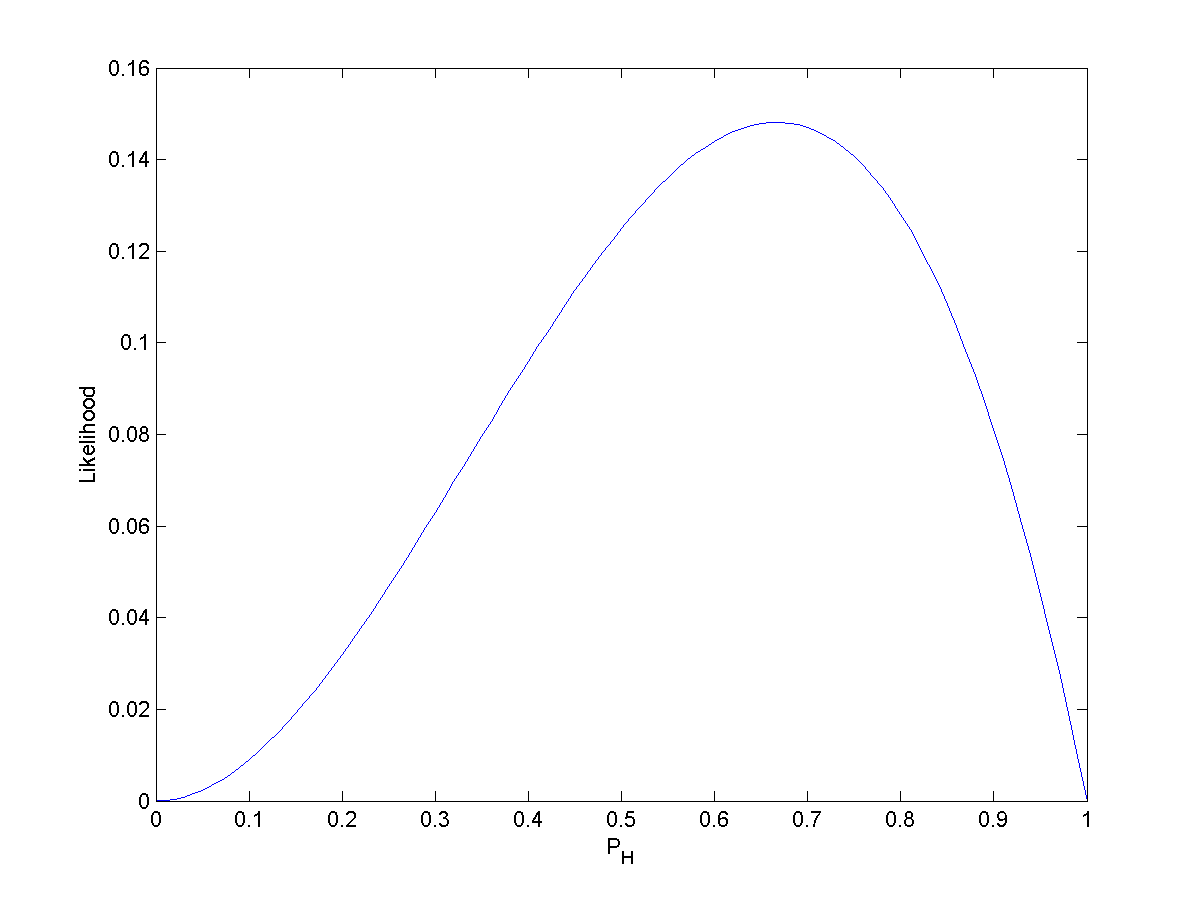
\includegraphics[width=0.8\linewidth]{likelihood_coin_hht.png}
  \caption{The likelihood function ($p^2_H(1-p_H)$) for the probability of a
    coin landing heads-up (without prior knowledge of the coin's fairness),
    given that we have observed HHT.}%
  \label{fig:likelihood_coin_hht}
\end{figure}


\end{document}
